\normaltrue
\correctionfalse

%\UPSTIidClasse{12} % 11 sup, 12 spé
%\newcommand{\UPSTIidClasse}{12}

\exer{Automate d’exploration de l’hémostase $\star$ \label{DYN:02:C2:09:1D:61:02}}
\setcounter{question}{0}\marginnote{\xpComp{DYN}{01}}%\UPSTIcompetence[2]{C2-09}
\index{Compétence C2-09}\index{Compétence DYN-01}
\index{Principe fondamental de la dynamique}
\index{PFD}
%\index{Mécanisme à 1 rotation}
\index{Automate d’exploration de l’hémostase}
\ifcorrection
\else
\marginnote{\textbf{Pas de corrigé pour cet exercice.}}
\fi


\ifprof
\else
Le principe de la chronométrie consiste à mesurer la variation de l’amplitude d’oscillation d’une
bille placée dans la cuvette de mesure (\autoref{61_01}).%(figures 10 et 11).

\begin{marginfigure}\centering
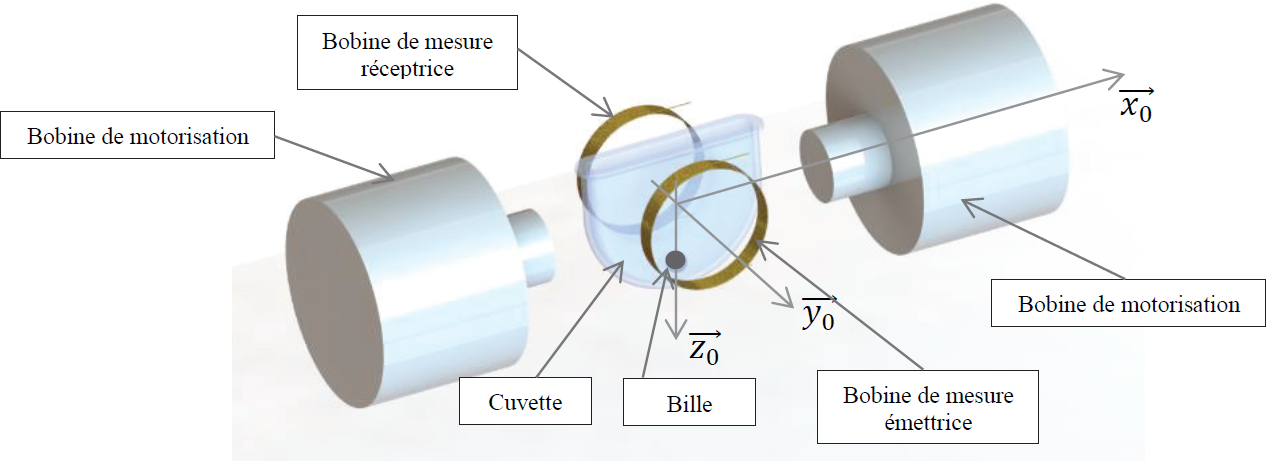
\includegraphics[width=\linewidth]{61_01}
\caption{\label{61_01} Ensemble cuvette + bille avec bobines motrices et bobines de mesure}
\end{marginfigure}

La bille, roulant sans glisser sur le fond cylindrique de la cuvette, est mise en mouvement par un
champ magnétique variable induit par deux bobines motrices placées de part et d’autre de la tête de
mesure.
L’amplitude des oscillations est mesurée par deux autres bobines, l’une émettrice, l’autre réceptrice.
Après amplification du signal mesuré, on obtient un signal quasi-sinusoïdal, reflet de l’oscillation
de la bille. A viscosité constante, on obtient un balancement pendulaire constant de la bille. Quand
la viscosité augmente (phénomène de coagulation), l’amplitude d’oscillation de la bille varie.
Pour chaque mesure, le champ magnétique est ajusté en fonction de la viscosité initiale du milieu et
du type de test.

%Dans un premier temps, on se propose de modéliser le comportement de la bille pour en déduire le
%réglage de la commande des bobines motrices. (partie 3.3, page 9).
%Dans un second temps, un algorithme détermine le temps de coagulation à partir de l’amplitude des
%oscillations. Celui-ci sera défini paragraphe 4.1, page 14 (partie informatique).


%\subsubsection{Hypothèses de calculs}
Le schéma de calcul est donné \autoref{61_02}.


\begin{marginfigure}
\centering
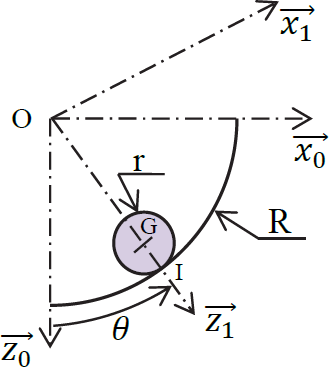
\includegraphics[width=\linewidth]{61_02}
\caption{\label{61_02} Bille en contact avec le rail de la cuvette}
\end{marginfigure}

Hypothèses :
\begin{itemize}
\item la bille de masse $m$, de centre de masse $G$, de rayon $r$,
roule sans glisser sur un rail circulaire de rayon $R$ dans
le plan $\left(O,\vect{x_0},\vect{y_0}\right)$;
\item $I$ est le point de contact entre la bille et le rail circulaire ;
\item la position de la bille sur le rail est repérée par : $\theta = \left(\vect{z_0},\vect{z_1} \right)= \left(\vect{x_0},\vect{x_1} \right)$.
\end{itemize}

On note :
\begin{itemize}
\item $\torseurstat{T}{\text{rail}}{\text{bille}} = \torseurl{-N_I\vect{z_1}+T_I\vect{x_1}}{\vect{0}}{I}$, le torseur associé à l’action mécanique du rail sur la bille ;
\item $f$ le coefficient d’adhérence au contact bille/cuvette : $f=0,1$; 
\item $\torseurstat{T}{\text{bob}}{\text{bille}} = \torseurl{\vect{F}\left(\text{bob} \rightarrow \text{bille} \right)=F(t)\vect{x_0}}{\vect{0}}{G}$, le torseur associé à l’effort résultant des deux bobines de motorisation sur la bille, avec $F(t)=F_0\sin\left(\omega_{\text{bob}}(t)\right)$ ;
\item $\torseurstat{T}{\text{fluide}}{\text{bille}} = \torseurl{\vect{F}\left(\text{fluide} \rightarrow \text{bille} \right)=-f_v\vectv{G}{\text{bille}}{0}}{\vect{0}}{G}$, le torseur associé à
l’action du fluide sur la bille induite par la viscosité. On se place dans l’hypothèse
simplificatrice d’un écoulement laminaire pour lequel le modèle de Stokes est applicable : le
coefficient de frottement visqueux vaut alors $f_v = 6\pi r \eta $  où $\eta$ est la viscosité du sang qui
varie lors de la coagulation ;
\item $\torseurstat{T}{g}{\text{bille}} = \torseurl{mg\vect{z_0}}{\vect{0}}{G}$, le torseur associé à l’action de la pesanteur sur la bille ;
\item $\torseurcin{V}{\text{bille}}{0} = \torseurl{\vecto{\text{bille}}{0}=\omega_b \vect{y_0}}{\vectv{G}{\text{bille}}{0}=v\vect{x_1}}{G}$, le torseur cinématique de la bille par rapport au rail 0 ;
\item $J = \dfrac{2}{5}mr^2$, le moment d’inertie de la bille autour de l’axe $\axe{G}{y_0}$;
\item $R=||\vect{OI}||$, le rayon du rail, $r=||\vect{GI}||$, le rayon de la bille.
\end{itemize}
On notera $F(p)$ la transformée de Laplace de la fonction $f(t)$ où $p$ représente la variable de
Laplace.
\fi

\question{En exprimant la condition de roulement sans glissement en $I$, déterminer $\omega_b$ et $v$, les
composantes du torseur cinématique en $G$ de la bille par rapport au rail 0, en fonction de $\dot{\theta}$, $r$ et $R$.}
\ifprof
\begin{itemize}
\item On isole la bille. 
\item On réalise le bilan des actions mécaniques :
\begin{itemize}
\item $\torseurstat{T}{\text{rail}}{\text{bille}} = \torseurl{-N_I\vect{z_1}+T_I\vect{x_1}}{\vect{0}}{I}$ $= \torseurl{-N_I\vect{z_1}+T_I\vect{x_1}}{rT_I\vect{y_1}}{G}$.
\item $\torseurstat{T}{\text{bob}}{\text{bille}} = \torseurl{\vect{F}\left(\text{bob} \rightarrow \text{bille} \right)=F(t)\vect{x_0}}{\vect{0}}{G}$.
\item $\torseurstat{T}{\text{fluide}}{\text{bille}} = \torseurl{\vect{F}\left(\text{fluide} \rightarrow \text{bille} \right)=-f_v\vectv{G}{\text{bille}}{0}}{\vect{0}}{G}$.
\item $\torseurstat{T}{g}{\text{bille}} = \torseurl{mg\vect{z_0}}{\vect{0}}{G}$.
\end{itemize}
\item On calcule le torseur dynamique de la bille $\torseurdyn{\text{bille}}{0}=\torseurl{m\vectg{G}{\text{bille}}{0}}{-J\dfrac{R-r}{r}\ddot{\theta}\vect{y_0}}{G}$ avec $\vectg{G}{\text{bille}}{0} = \dfrac{\dd \vectv{G}{\text{bille}}{0}}{\dd t} = (R-r)\ddot{\theta}\vect{x_1} - (R-r)\dot{\theta}^2\vect{z_1}$.
\end{itemize}

En appliquant le TRD à la bille en projection sur $\vect{z_1}$, on a : 
$-N_I+F(t)\vect{x_0}\cdot\vect{z_1} +mg\vect{z_0}\cdot\vect{z_1} = - m(R-r)\dot{\theta}^2$
$\Longleftrightarrow -N_I+F(t)\sin\theta +mg\cos\theta = - m(R-r)\dot{\theta}^2 $.


En appliquant le TMD à la bille, en $G$, en projection sur $\vect{y_0}$, on a : 
$rT_1 = -J\dfrac{R-r}{r}\ddot{\theta}$
$\Longleftrightarrow rT_1 = -\dfrac{2}{5}mr^2 \dfrac{R-r}{r}\ddot{\theta}$
$\Longleftrightarrow T_1 = \dfrac{2}{5}m(r-R)\ddot{\theta}$.

\else
\fi

\question{En justifiant clairement la démarche et les théorèmes utilisés : montrer que les efforts normal $N_I$ et tangentiel
 $T_I$ du rail sur la bille sont liés à l’angle $\theta$ par les équations suivantes :}
$N_I = F(t)\sin \theta +mg \cos \theta + m\left(R-r\right)\dot{\theta}^2$
et $T_I = \dfrac{2}{5}m\left(r-R\right)\ddot{\theta}$.
\ifprof
En appliquant le TRD à la bille en projection sur $\vect{x_1}$, on a : 
$T_I+F(t)\vect{x_0}\cdot\vect{x_1} +mg\vect{z_0}\cdot\vect{x_1}-f_v \left(R-r\right)\dot{\theta} =  m(R-r)\ddot{\theta}$
$\Longleftrightarrow  T_I+F(t)\cos\theta-mg\sin\theta -f_v \left(R-r\right)\dot{\theta} =  m(R-r)\ddot{\theta}$.

En utilisant la question précédente, on a alors 
$\dfrac{2}{5}m(r-R)\ddot{\theta}+F(t)\cos\theta-mg\sin\theta -f_v \left(R-r\right)\dot{\theta} =  m(R-r)\ddot{\theta}$

$\Longleftrightarrow F(t)\cos\theta = mg\sin\theta  + f_v \left(R-r\right)\dot{\theta} + \dfrac{7}{5}m(R-r)\ddot{\theta}$

(Signe à revoir ?).
\else
\fi


\question{En justifiant clairement la démarche et les théorèmes utilisés, montrer que $\dfrac{7}{5}m\left(r-R\right)\ddot{\theta}
+f_v\left(r-R\right)\dot{\theta}+mg\sin\theta=F(t)\cos\theta$.}
\ifprof
Si $\theta$ est petit $\dfrac{7}{5}m\left(r-R\right)\ddot{\theta} +f_v\left(r-R\right)\dot{\theta}+mg\theta=F(t)$. 
En passant dans le domaine de Laplace, on a $\dfrac{7}{5}m\left(r-R\right)p^2{\theta(p)} +f_v\left(r-R\right)p {\theta(p)}+mg\theta(p)=F(p)$
soit $H(p)=\dfrac{1}{\dfrac{7}{5}m\left(r-R\right)p^2 +f_v\left(r-R\right)p +mg}$

$ = \dfrac{\dfrac{1}{mg}}{\dfrac{7}{5g}\left(r-R\right)p^2 +\dfrac{f_v}{mg}\left(r-R\right)p +1}$.

On a donc $K_S = \dfrac{1}{mg}$, $\omega_0 = \sqrt{\dfrac{5g}{7\left(r-R\right)}}$,
$\dfrac{2 \xi }{\omega_0} = \dfrac{f_v\left(r-R\right)}{mg}$ soit $\xi =\dfrac{f_v\left(r-R\right)}{2mg}\sqrt{\dfrac{5g}{7\left(r-R\right)}} =\dfrac{f_v}{2mg}\sqrt{\dfrac{5g\left(r-R\right)}{7}} $

\else
\fi


\ifprof
\else

\marginnote{Corrigé voir \ref{DYN:02:C2:09:1D:61:02}.}

\fi